\section{Theorie}
\label{sec:Theorie}
\subsection{Magnetische Momente und Drehimpulse}
Ein Hüllenelektron besitzt zwei Drehimpulse, den Spin $\vec{s}$ und den Bahndrehimpuls $\vec{l}$.
Deren Beträge sind wie folgt definiert durch die Quantenzahlen $\textit{l}$ und $s$:
\begin{align}
  |\vec{l}|&=\sqrt{\textit{l}(\textit{l}+1)\hbar}\,\,\,\,\,\text{mit $\textit{l}=0,1,...n-1$ }\\
  |\vec{s}|&=\sqrt{s(s+1)\hbar}\,\,\,\,\,\text{mit $s=\frac{1}{2}$}\
\end{align}
Den beiden Drehimpulsen kann ein magnetischen Moment zugeordnet werden:
\begin{align}
  \vec{\mu_\mathrm{\textit{l}}}&=-\mu_\mathrm{B}\sqrt{\textit{l}(\textit{l}+1)}\vec{\textit{l}_\mathrm{e}}\\
  \vec{\mu_\mathrm{s}}&=-\mu_\mathrm{B} g_\mathrm{s}\sqrt{s(s+1)}\vec{s_\mathrm{e}}\\
\end{align}
Es besteht eine Proportionalität zum Bohrschen-Magneton $\mu_\mathrm{B}:=\frac{1}{2}e_\mathrm{0}\frac{\hbar}{m_\mathrm{0}}$
(mit $e_\mathrm{0}$ der Elektronenladung und $m_\mathrm{0}$ der Elektronenmasse).
Die magnetische Anomalie des Elektons sorgt für den zusätzlichen Faktor $g_\mathrm{s}=2$
im magnetischen Moment des Spins.

\subsection{Wechselwirkung der Drehimpulse}
Die Wechselwirkung von Bahndrehimpulsen und Spins kann auf komplizierte Weise ablaufen.
In der Natur treten zwei Grenzfälle auf, die im Folgenden thematisiert werden:\\
\\
\textbf{1.Fall:} Bei leichten Atomen setzen sich die einzelnen Bahndrehimpulse und Spins
zu einem Gesamtbahndrehimpuls der Elektronenhülle $\vec{L}=\sum_i l_i$
bzw. Gesamtspin der Elektronenhülle $\vec{S}=\sum_i s_i$ zusammen.
Der Gesamtdrehimpuls hat den Betrag
\begin{align*}
 |\vec{L}|=\sqrt{L(L+1)\hbar}
\end{align*}
und ist eine quantisierte Größe:
$L$ ist ganzzahlig und nimmt die Werte $0,1,2 ,\ \text{oder} ,\ 3$ an.
Ähnlich sieht es bei dem Gesamtspin aus, der Betrag entspricht
\begin{align*}
 |\vec{S}|=\sqrt{S(S+1)\hbar}
\end{align*}
mit der Quantenzahl $S$. Die kann Werte von $\frac{N}{2} ,\ \text{bis} ,\ 0$
($N$ ist die Anzahl der Elektronen in den nicht abgeschlossenen Schalen)
in halbzahligen Schritten annehmen.
Diese beiden Größen koppeln zu einem Gesamtdrehimpuls der Elektronenhülle $\vec{J}$ über die sogenannte LS-Kopplung:
\begin{align}
  \vec{J}=\vec{L}+\vec{S} ,\,\,\,\,\, \text{mit dem Betrag}\,\,\,\,\,|\vec{J}|=\sqrt{J(J+1)\hbar}.
\end{align}\\
\textbf{2.Fall:} Bei schweren Atomen ist die Wechselwirkung zwischen dem Spin und
Bahndrehimpuls eines einzelnen Elektrons größer als zwischen allen Elektronen.
Es entsteht kein Gesamtbahndrehimpuls bzw. Gesamtspin.
Bahndrehimpulse $\vec{\textit{l}_\mathrm{i}}$ und Spins $\vec{s}_\mathrm{i}$ der einzelnen Elektronen ergeben
die Gesamtdrehimpulse $\vec{j}_\mathrm{i}=\vec{\textit{l}_\mathrm{i}}+\vec{s}_\mathrm{i}$ der Elektronen.
Erst die Summe aller $\vec{j}_\mathrm{i}$ ergibt den Gesamtdrehimpuls der Elektronenhülle:
\begin{align}
\vec{J}=\sum_i \vec{j}_i.
\end{align}\\
Für mittelschwere Atome besteht ein fließender Übergang.
\\
Das gesamte magnetische Moment $\vec{\mu}$ zum Gesamtdrehimpuls $\vec{J}$ ergibt sich aus der Vektorsumme der magnetischen Momente
\begin{align*}
 \vec{\mu_\mathrm{L}}&=\mu_\mathrm{B}\sqrt{L(L+1)}\
 \intertext{und}\
 \vec{\mu_\mathrm{S}}&=\mu_\mathrm{B}g_\mathrm{s}\sqrt{S(S+1)}.
\end{align*}
Die Richtungen von $\vec{\mu}$ und $\vec{J}$ fallen nicht zusammen, jedoch kann
gezeigt werden, dass der zu $\vec{J}$ parallele Anteil von $\vec{\mu}$ beiträgt.
Diese und weitere Überlegungen führen zum Betrag des magnetischen Momentes:
\begin{align}
  |\vec{\mu}_\mathrm{J}|\approx \mu_\mathrm{B}\sqrt{J(J+1)}\underbrace{\frac{3J(J+1)+S(S+1)-L(L+1)}{2J(J+1)}}_{g_\mathrm{J}}
\end{align}
Hierbei bezeichnet $g_\mathrm{J}$ den Landé-Faktor.
Unter deim Einfluss eines B-Feldes nehmen die Winkel zwischen $\vec{\mu}$ und $\vec{B}$ Werte an,
bei denen die Komponente $\mu_\mathrm{J_\mathrm{z}}$ in Feldrichtung ein ganzzahliges Vielfaches
von $g_\mathrm{J}\mu_\mathrm{B}$ ergibt.
Diese sogenannte Richtungsquantelung kann ausgedrückt werden durch:
\begin{align}
  \mu_\mathrm{J_\mathrm{z}}= -mg_\mathrm{J}\mu_\mathrm{B},
\end{align}
die ganzzahlige größe $m$ beschreibt die Orientierungsquantenzahl und hat einen Wertevorrat von
$-J$ bis $J$.
Es existieren $2J+1$ Einstellungen des magnetischen Momentes relativ zur äußeren Feldrichtung und
damit eine Aufspltung eines Nivaus in $2J+1$ Unterniveaus.
\subsection{Auswahlregeln}
Zwischen den Zuständen sind Übergänge unter der Emission eines Photons möglich.
Die Energie des Photos, damit auch die Wellenlänge der messbaren Spektrallinie,
entspricht dabei der Energiedifferenz der beiden Zustände.
%%%%%%%%%%%%%%%%%%%%%%%%%%%%%%%Rechnung
Aus Rechnungen folgen Auswahlregeln für die Übergänge.
Übergänge zwischen den Zuständen sind danach nur möglich wenn die
Orientierungsquantenzahl $m$ sich um $\pm 1$ oder gar nicht ändert:
\begin{align*}
  \Delta m = 0,\pm 1.
\end{align*}
\subsection{Normaler Zeemann-Effekt}
Beim normalen Zeemann-Effekt entspricht $S=0$ für alle $J:g_\mathrm{j}=1$,
dies bedeutet die Unabhängigkeit der Verschiebung der Energieniveaus von den Quantenzahlen.
Für jedes $L$ und $S$ gilt:
\begin{align}
  \Delta E=m\mu_\mathrm{B}B ,\,\,\,\,\ \text{für}\,\-J < m < J.
\end{align}
Es findet die Aufspaltung in die äquidistanten Unterniveaus statt, dies geschiecht auch im Angeregten Zustand.
Ein Übergang nach den Auswahlregeln kann somit stattfinden.
Die Aufspaltung und möglichen Übergänge sind in Abbildung \ref{fig:normal} dargestellt.
Die Übergänge lassen sich anhand ihrer Polarisation kategorisieren:
\begin{itemize}
  \item{$\sigma^+$-Übergang: $\Delta m_\mathrm{J}=+1$  entspricht rechtszirkularer Polarisation um das Magnetfeld}
  \item{$\sigma^-$-Übergang: $\Delta m_\mathrm{J}=-1$) entspricht linkszirkularer Polarisation um das Magnetfeld }
  \item{$\pi$-Übergang: $\Delta m_\mathrm{J}=0$ entspricht linearer Polarisation in Magnetfeldrichtung}
\end{itemize}
\begin{figure}
   \centering
    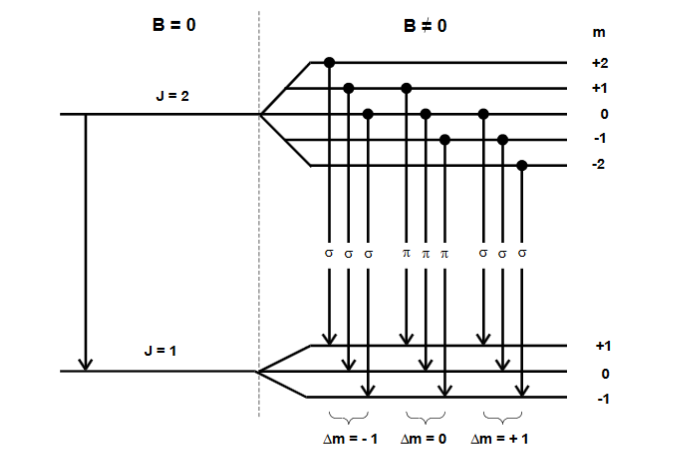
\includegraphics[width=0.8\textwidth]{normal.PNG}
    \caption{Aufspaltung und mögliche Übergänge beim Zeemann-Effekt.\cite{skript}}
    \label{fig:normal}
\end{figure}
Beim normalen Zeemann-Effekt findet grundsätzlich eine Aufspalung in ein Tripplet auf, weil die Energiedifferenzen
innerhalb einer Gruppe mit konstantem $\Delta m$ gleich sind.
Aufgrund der Polarisation sind die Lienien nicht aus jeder Richtung beobachtbar.
Die $\pi$-Linie liegt mit maximaler Intensität senkrecht zur Feldrichtung vor und ist in Feldrichtiung nicht beobachtbar.
Die $\sigma$-Linien erscheinen, senkrecht zur Feldrichtung, ebenfalls linear Polarisiert aber senkrecht zur $\pi$-Linie.
Die Abbildung \ref{fig:aufspaltungsbild} zeigt das Aufspaltungsbild einer Spektrallinie.
\begin{figure}
   \centering
    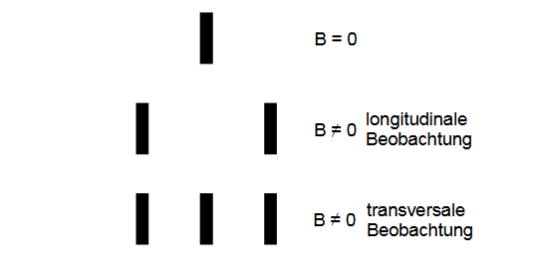
\includegraphics[width=0.7\textwidth]{aufspaltungsbild.PNG}
    \caption{Das Aufspltungsbild einer Spektrallinie.\cite{skript}}
    \label{fig:aufspaltungsbild}
\end{figure}
\subsection{Anomaler Zeemann-Effekt}
Bei dem anomalen Zeemann-Effekt gilt $S \neq 0$ und damit hängen die Energiedifferenzen vom Spin ab.
In diesem Fall ist $g_\mathrm{j}$ nicht automatisch $1$, sondern nimmt verschiedene Werte an.
Die Energieverschiebung ist dann gegeben durch:
\begin{align}
  \Delta E= [m_\mathrm{1}g_\mathrm{J}(L_\mathrm{1},S_\mathrm{1},J_\mathrm{1})]-m_\mathrm{2}g_\mathrm{J}(L_\mathrm{2},S_\mathrm{2},J_\mathrm{2}).
\end{align}
Die Indizes geben die Zordnung zu den Niveaus an.
Die Aufspaltung ist wesentlich Linienreicher und ist in Abbildung \ref{fig:anomal} dargestellt.
\begin{figure}
   \centering
    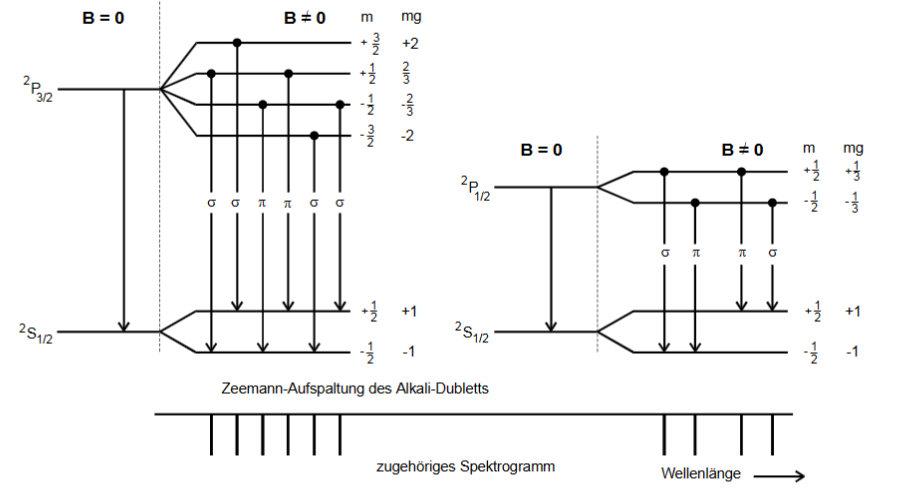
\includegraphics[width=0.8\textwidth]{anomal.PNG}
    \caption{Die Aufspaltung beim anomalen Zeemann-Effekt.\cite{skript}}
    \label{fig:anomal}
\end{figure}
\subsection{Lummer-Gehrcke-Platte}
In diesem Versuch wird zur Sichtbarmachung der Aufspaltung eine Lummer-Gehrke-Platte genutzt.
An dieser Stelle folgt ein kurze Beschreibung der Funktionsweise der Platte.
Eingestrahltes Licht wird innerhalb der Platte mehrfach reflektiert, dabei tritt bei
jeder Reflektion ein Teil des Lichts an der oberen und unteren Grenzfläche aus.
Dies ist in Abbildung $\ref{fig:platte}$ dargestellt.
\begin{figure}
   \centering
    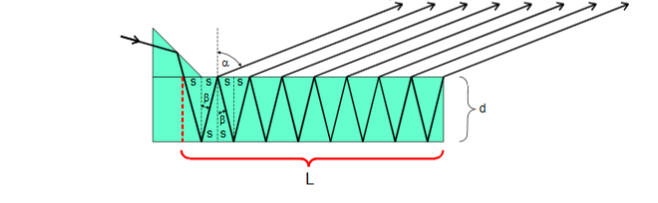
\includegraphics[width=0.9\textwidth]{platte.PNG}
    \caption{Der Strahlengang innerhalb der Lummer-Gehrcke-Platte.\cite{skript}}
    \label{fig:platte}
\end{figure}
Die Strahlen interferieren konstruktiv wenn die Bedingung $2d\cos{\theta}=n\lambda$
erfüllt ist. Hierbei ist $d$ die Dicke der Platte und $\lambda$ die Wellenlänge der Strahlung.
Bei eingeschaltetem Magnetfeld verändert sich die Wellenlänge um $\delta\lambda$ und
die Interferenzstreifen verschieben sich um $\delta s$.
Von Bedeutung sind die beiden Größen Dispersionsgebiet und Auflösungsvermögen.
Das Dispersionsgebiet gibt den Wellenlängendifferenzbereich an, in dem die
Interferenzstreifen sich nicht überlagern:
\begin{align}
  \Delta\lambda_\mathrm{D}=\frac{\lambda^2}{2d}\sqrt{\frac{1}{n^2-1}} \label{eqn:dispersionsgebiet}.
\end{align}
Das Auflösungsvermögen ist durch folgende Beziehung zwischen Brechungsindex $n$,
der Plattenlänge $L$ und der Wellenlänge gegeben:
\begin{align}
  A=\frac{L}{\lambda}(n^2-1)\label{eqn:aufloesung}.
\end{align}
